\chapter{Sicurezza e privacy}\label{ch-07}

\lecturemeta{Capitolo originale: 7 --- Security and Privacy \quad\textbullet\quad Antonio Brogi}{Appunti di Emiliano Sescu (github.com/Faxatos), cap. 7}

La sicurezza del software è una priorità sia per chi sviluppa il
prodotto sia per chi lo usa, perché un attacco può causare danni a
entrambi. La Fig. 7.1 mostra i tipi principali di minaccia; alcuni
attacchi li combinano (ad esempio un \textbf{ransomware} colpisce
l'integrità dei dati, ma di conseguenza anche la disponibilità del
sistema).

\begin{figure}[H]
\centering
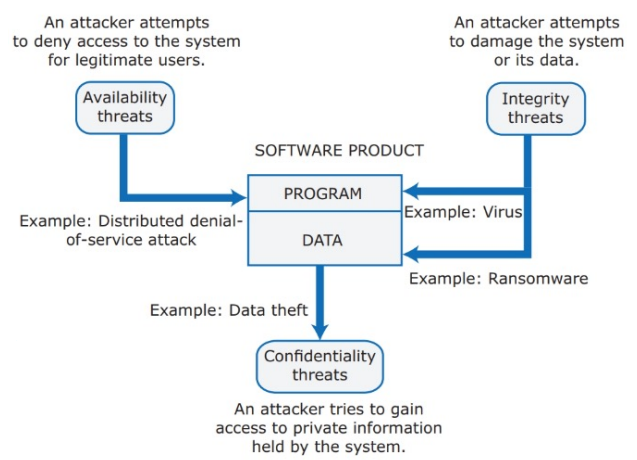
\includegraphics[width=0.80\linewidth,height=0.45\textheight,keepaspectratio]{images/07-sicurezza_fig7-1_minacce.png}
\caption{I tipi principali di minacce alla sicurezza.}
\end{figure}

\begin{boxtip}{Le tre minacce in breve}

\begin{itemize}
\tightlist
\item
  \textbf{Disponibilità} (\emph{availability}): impedire agli utenti
  legittimi di usare il sistema.
\item
  \textbf{Integrità} (\emph{integrity}): danneggiare il sistema o i suoi
  dati.
\item
  \textbf{Riservatezza} (\emph{confidentiality}): accedere a
  informazioni private.
\end{itemize}

\end{boxtip}

La sicurezza riguarda \textbf{tutto il sistema}: il software applicativo
dipende dal sistema operativo, dal web server, dal runtime del
linguaggio, dal database, dai framework, dagli strumenti, ecc. Un
attacco può colpire qualsiasi livello dell'infrastruttura, a partire
dalla rete.

Alcune attività di gestione del sistema per mantenerlo sicuro:

\begin{itemize}
\tightlist
\item
  \textbf{Standard e procedure di autenticazione e autorizzazione},
  perché tutti gli utenti abbiano un'autenticazione forte e permessi di
  accesso impostati bene.
\item
  \textbf{Gestione dell'infrastruttura}: tenere configurato bene il
  software di base e applicare subito gli aggiornamenti di sicurezza che
  correggono le vulnerabilità.
\item
  \textbf{Monitoraggio regolare degli attacchi}, per accorgersene presto
  e attivare strategie di difesa che ne limitino gli effetti.
\item
  \textbf{Politiche di backup}, per avere copie integre di programmi e
  dati da ripristinare dopo un attacco.
\end{itemize}

\section{Attacchi e difese}\label{attacchi-e-difese}

\subsection{Injection}\label{injection}

Un attacco di \textbf{injection} avviene quando un utente
malintenzionato usa un campo di input valido per inserire \textbf{codice
malevolo} o \textbf{comandi per il database} che danneggiano il sistema.

\begin{itemize}
\tightlist
\item
  \textbf{Buffer overflow}: una delle classi di attacco più comuni.
  L'attaccante costruisce con cura una stringa di input che contiene
  istruzioni eseguibili e sovrascrive la memoria. Se viene sovrascritto
  l'indirizzo di ritorno di una funzione, il controllo passa al codice
  malevolo. Succede ad esempio con sistemi operativi e librerie scritti
  in C/C++, che non controllano se gli accessi agli array restano nei
  limiti.
\item
  \textbf{SQL injection}: possibile quando l'input dell'utente diventa
  parte di un comando SQL.
\end{itemize}

La contromisura più semplice è \textbf{controllare la validità
dell'input}.

\begin{boxexample}{SQL injection}

Se il codice costruisce la query come
\texttt{"SELECT\ *\ FROM\ users\ WHERE\ name\ =\ \textquotesingle{}"\ +\ input\ +\ "\textquotesingle{}"}
e l'utente scrive
\texttt{\textquotesingle{}\ OR\ \textquotesingle{}1\textquotesingle{}=\textquotesingle{}1},
la condizione diventa sempre vera e la query restituisce tutti gli
utenti. Oltre a validare l'input, la difesa standard è usare
\textbf{query parametrizzate} (\emph{prepared statement}).

\end{boxexample}

\subsection{Session hijacking}\label{session-hijacking}

Molte applicazioni usano il concetto di \textbf{sessione}: un periodo in
cui l'autenticazione dell'utente con l'applicazione web resta valida. Di
solito si realizza con dei \textbf{cookie di sessione} (token) che il
server dà al client e che il client rimanda a ogni richiesta HTTP, così
l'utente non deve autenticarsi di nuovo a ogni interazione. La sessione
si chiude quando l'utente fa logout o quando scade (\emph{timeout}).

Nel \textbf{session hijacking} (furto di sessione) l'attaccante si
procura un cookie di sessione valido per \textbf{fingersi un utente
legittimo}. Può ottenerlo con un attacco di cross-site scripting o
osservando il traffico (facile su Wi-Fi non protette e con dati non
cifrati). L'attacco può essere:

\begin{itemize}
\tightlist
\item
  \textbf{attivo}: l'attaccante compie azioni sul server al posto
  dell'utente;
\item
  \textbf{passivo}: l'attaccante si limita a osservare il traffico
  client-server in cerca di informazioni utili (password, numeri di
  carta di credito, \ldots).
\end{itemize}

Difese: \textbf{cifrare il traffico} client-server (es. HTTPS), usare
l'\textbf{autenticazione a più fattori} per confermare azioni nuove e
potenzialmente dannose, usare \textbf{timeout di sessione} abbastanza
brevi.

\subsection{Cross-site scripting (XSS)}\label{cross-site-scripting-xss}

Il \textbf{cross-site scripting} è un'altra forma di injection:
l'attaccante aggiunge \textbf{codice JavaScript malevolo} alla pagina
web che il server manda al client. Lo script viene eseguito quando la
pagina è mostrata nel browser della vittima, con l'obiettivo di rubare
informazioni del cliente o dirottarlo su un altro sito. Può anche rubare
i cookie, rendendo possibile il session hijacking.

\begin{figure}[H]
\centering
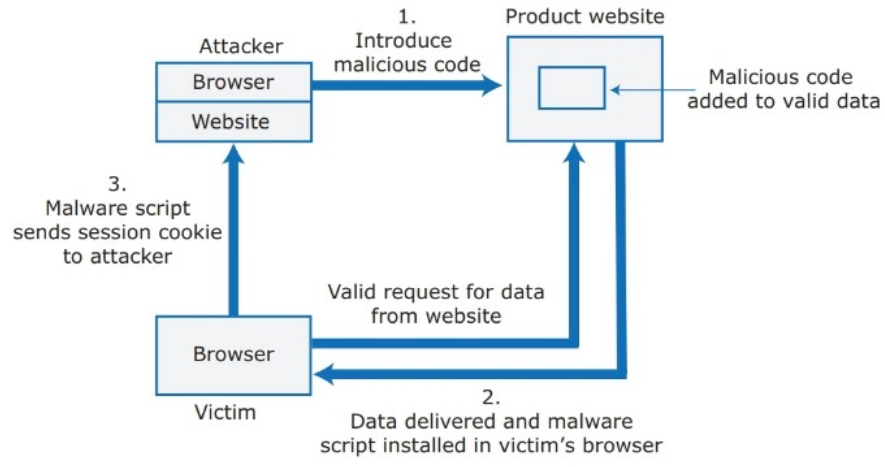
\includegraphics[width=0.93\linewidth,height=0.45\textheight,keepaspectratio]{images/07-sicurezza_fig7-2_cross-site-scripting.png}
\caption{Un attacco di cross-site scripting.}
\end{figure}

Difese: \textbf{validare l'input} (dei form), \textbf{controllare i dati
presi dal database} prima di inserirli nella pagina generata, usare il
comando HTML di \textbf{``encode''} (così le informazioni aggiunte alla
pagina non sono eseguibili).

\subsection{Denial of Service (DoS)}\label{denial-of-service-dos}

Gli attacchi \textbf{Denial of Service} (DoS) vogliono rendere il
sistema \textbf{inutilizzabile} per l'uso normale. Di solito si usano
molti computer distribuiti (spesso infettati e controllati
dall'attaccante) che mandano centinaia di migliaia di richieste a
un'applicazione web (\textbf{DDoS}, \emph{Distributed DoS}). Lo scopo è
sabotare il fornitore del servizio o chiedere un riscatto.

Contromisure:

\begin{itemize}
\tightlist
\item
  software specializzati che \textbf{rilevano e scartano} i pacchetti in
  arrivo, evitando di essere sommersi dalle richieste;
\item
  \textbf{blocchi temporanei} degli utenti (es. bloccare un utente dopo
  ripetuti tentativi di login falliti con la sua email);
\item
  \textbf{tracciamento degli indirizzi IP} (es. applicare il blocco solo
  se i tentativi falliti arrivano da indirizzi IP insoliti).
\end{itemize}

\subsection{Brute force}\label{brute-force}

L'attaccante ha solo una parte delle informazioni (es. un nome utente
valido ma non la password) e prova ripetutamente a indovinare la parte
mancante, ad esempio con un generatore di stringhe che crea tutte le
combinazioni possibili di lettere e numeri.

Difese: convincere (cioè obbligare) gli utenti a usare \textbf{password
lunghe}, che non siano nel dizionario né parole comuni. Un ulteriore
livello di sicurezza è l'\textbf{autenticazione a due fattori}.

\section{Autenticazione e
autorizzazione}\label{autenticazione-e-autorizzazione}

\subsection{Autenticazione}\label{autenticazione}

\begin{boxdefinition}{Autenticazione}

L'\textbf{autenticazione} serve a garantire che gli utenti del sistema
siano \textbf{davvero chi dicono di essere}.

\end{boxdefinition}

Ci sono tre approcci principali:

\begin{itemize}
\tightlist
\item
  \textbf{Basata sulla conoscenza} (\emph{knowledge-based}): l'utente
  fornisce informazioni segrete e personali scelte alla registrazione
  (es. una password). Ha diversi punti deboli: password poco sicure;
  \textbf{phishing} (l'utente clicca un link in una email che porta a un
  sito falso che raccoglie login e password); stessa password usata
  ovunque; password dimenticate spesso (serve un meccanismo di recupero,
  che è una possibile vulnerabilità se le credenziali sono state
  rubate). Si può rendere più sicura obbligando a usare password forti e
  aggiungendo domande personali per il recupero.
\item
  \textbf{Basata sul possesso} (\emph{possession-based}): l'utente ha un
  \textbf{dispositivo fisico} collegato al sistema che genera o mostra
  informazioni note al sistema (es. un codice inviato al numero di
  telefono, o un dispositivo dedicato che genera codici usa e getta).
\item
  \textbf{Basata sugli attributi} (\emph{attribute-based}): usa una
  caratteristica \textbf{biometrica} unica dell'utente (impronta
  digitale, volto).
\end{itemize}

Se il sistema conserva informazioni riservate, la buona pratica è
l'\textbf{autenticazione a più fattori} (\emph{multi-factor}, es.
password e poi un codice ricevuto sul cellulare), che aggiunge un
livello di sicurezza.

Di solito gli sviluppatori non scrivono l'autenticazione da zero ma
usano librerie e toolkit già pronti (es.
\href{https://oauth.net/2/}{OAuth}). Anche così, costruire un sistema di
autenticazione sicuro e affidabile richiede molto lavoro. Per questo
spesso l'autenticazione si \textbf{delega} a un \textbf{sistema di
identità federata}, cioè a un servizio esterno (es. Google, Facebook),
come in Fig. 7.3. Questi servizi sono collaudati e probabilmente molto
più sicuri di qualsiasi sistema fatto in casa. In più il fornitore del
prodotto non deve gestire un proprio database di password e può ottenere
altre informazioni sull'utente (se l'utente acconsente).

\begin{figure}[H]
\centering
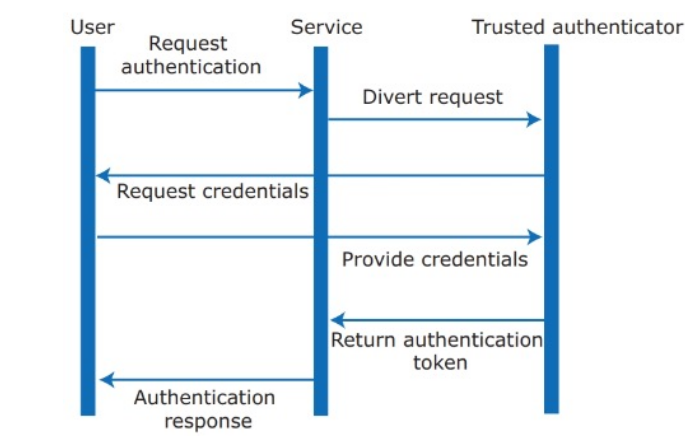
\includegraphics[width=0.85\linewidth,height=0.45\textheight,keepaspectratio]{images/07-sicurezza_fig7-3_identita-federata.png}
\caption{Diagramma di sequenza dell'identità federata.}
\end{figure}

Sui \textbf{dispositivi mobili} le regole cambiano, perché scrivere
password sulla tastiera del telefono è scomodo. Un'alternativa è
installare un \textbf{token di autenticazione} sul dispositivo, ma se il
telefono viene rubato o perso qualcun altro può accedere al prodotto.
Un'alternativa più sicura sono i \textbf{certificati digitali} personali
degli utenti, emessi da enti fidati.

\subsection{Autorizzazione}\label{autorizzazione}

\begin{boxdefinition}{Autorizzazione}

Mentre l'autenticazione verifica \textbf{chi è} l'utente,
l'\textbf{autorizzazione} controlla \textbf{a quali risorse} l'utente
può accedere.

\end{boxdefinition}

Nei prodotti multiutente serve un \textbf{controllo degli accessi}, con
una politica che rispetti le regole di protezione dei dati e limiti
l'accesso ai dati personali (anche per evitare cause legali in caso di
furto di dati).

Un modo diffuso per implementare la politica di accesso sono le
\textbf{Access Control List (ACL)}:

\begin{itemize}
\tightlist
\item
  gli utenti sono divisi in \textbf{gruppi}, e questo riduce molto la
  dimensione delle ACL;
\item
  gruppi diversi possono avere diritti diversi su risorse diverse;
\item
  le \textbf{gerarchie di gruppi} permettono di assegnare diritti a
  sottogruppi o a singoli utenti.
\end{itemize}

\begin{figure}[H]
\centering
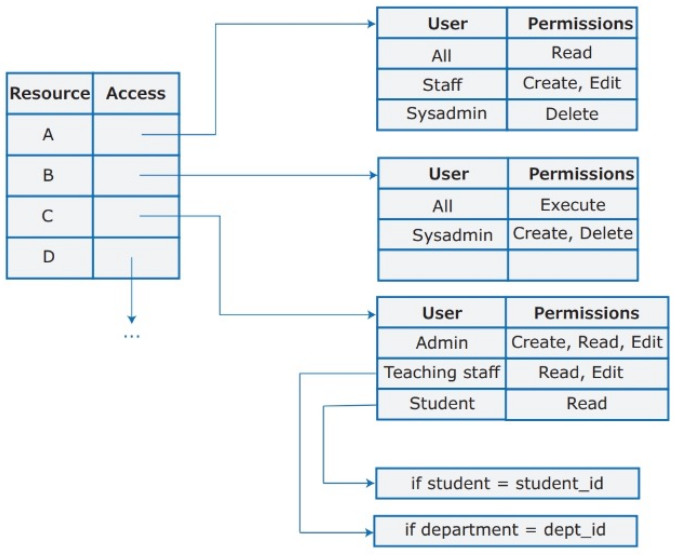
\includegraphics[width=0.85\linewidth,height=0.45\textheight,keepaspectratio]{images/07-sicurezza_fig7-4_access-control-list.png}
\caption{Esempio di Access Control List.}
\end{figure}

\section{Crittografia}\label{crittografia}

La \textbf{crittografia} (\emph{encryption}) rende un testo illeggibile
applicandogli una trasformazione algoritmica. Il testo viene cifrato con
una chiave segreta, viaggia su canali non sicuri e, quando arriva a
destinazione, viene \textbf{decifrato} con la stessa chiave o con
un'altra.

Le tecniche moderne sono considerate ``praticamente inattaccabili'' con
la tecnologia di oggi, anche se la storia insegna che una cifratura
apparentemente inattaccabile può diventare attaccabile con nuove
tecnologie (cosa succederà quando i computer quantistici saranno in
commercio?).

Esistono due grandi categorie:

\begin{itemize}
\tightlist
\item
  \textbf{Crittografia simmetrica}: è la più antica (usata da secoli) ma
  si usa ancora oggi. Usa \textbf{la stessa chiave} per cifrare e
  decifrare. Il suo punto debole è come \textbf{condividere la chiave}
  in modo sicuro.
\item
  \textbf{Crittografia asimmetrica}: usa \textbf{chiavi diverse} per
  cifrare e decifrare (una \textbf{pubblica} e una \textbf{privata}). È
  il metodo più sicuro, ma anche il più costoso in termini di calcolo.
\end{itemize}

\begin{boxtip}{Il meglio dei due mondi}

Di solito si \textbf{inizia} la comunicazione con la crittografia
asimmetrica solo per scambiarsi in modo sicuro una \textbf{chiave
simmetrica}, che poi si usa per il resto della comunicazione (più
veloce).

\end{boxtip}

\subsection{TLS}\label{tls}

Il \textbf{Transport Layer Security (TLS)} è un protocollo di sicurezza
molto diffuso per garantire privacy e sicurezza dei dati nelle
comunicazioni su Internet. L'uso principale è cifrare la comunicazione
tra applicazioni web e server, ad esempio quando un browser carica un
sito. Usato sopra HTTP dà \textbf{HTTPS}, ormai lo standard per i siti
web.

TLS serve anche a \textbf{verificare l'identità} dei web server tramite
i \textbf{certificati digitali} che il server manda al client. I
certificati sono emessi da enti fidati di verifica dell'identità
(\textbf{CA}, \emph{Certificate Authority}). La Fig. 7.5 mostra un
tipico handshake client-server.

\begin{figure}[H]
\centering
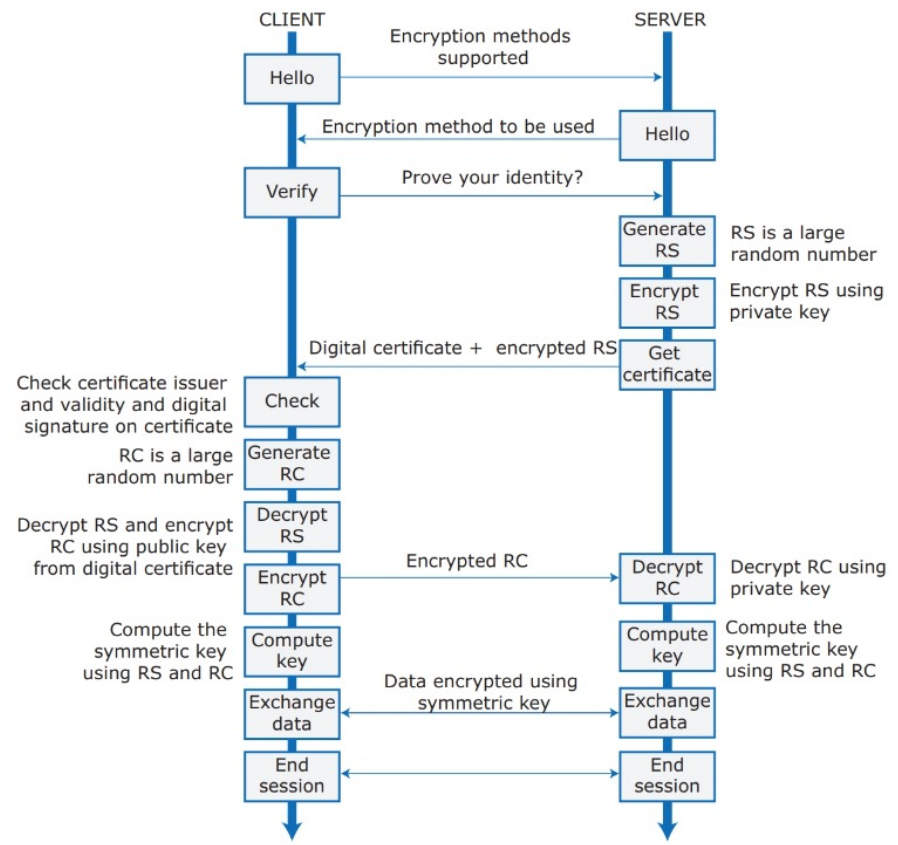
\includegraphics[width=0.80\linewidth,height=0.45\textheight,keepaspectratio]{images/07-sicurezza_fig7-5_handshake-tls.png}
\caption{Interazione TLS tra client e server per generare la chiave simmetrica
con cui scambiare i dati.}
\end{figure}

\subsection{Quando e dove cifrare}\label{quando-e-dove-cifrare}

I dati degli utenti si dividono in tre categorie:

\begin{itemize}
\tightlist
\item
  \textbf{Dati in transito} (\emph{in transit}): vanno \textbf{sempre
  cifrati}, per avere comunicazioni private.
\item
  \textbf{Dati a riposo} (\emph{at rest}, cioè salvati): vanno
  \textbf{sempre cifrati}, così in caso di attacco nessuno ottiene le
  informazioni degli utenti in chiaro.
\item
  \textbf{Dati in uso} (\emph{in use}, cioè in elaborazione): cifrarli e
  decifrarli \textbf{rallenta} i tempi di risposta del sistema.
\end{itemize}

La cifratura si può fare a quattro livelli:

\begin{itemize}
\tightlist
\item
  \textbf{Applicazione}: l'applicazione decide quali dati cifrare e li
  decifra subito prima di usarli. Costa in prestazioni (la sicurezza non
  è gratis) e richiede una gestione delle chiavi.
\item
  \textbf{Database}: il DBMS può cifrare l'intero database quando viene
  chiuso e decifrarlo quando viene riaperto, oppure cifrare solo singole
  tabelle o colonne.
\item
  \textbf{File}: il sistema operativo cifra i singoli file quando
  vengono chiusi e li decifra quando vengono riaperti.
\item
  \textbf{Supporto} (\emph{media}): il sistema operativo cifra i dischi
  quando vengono smontati e li decifra quando vengono rimontati (utile
  per portatili rubati o persi).
\end{itemize}

Tutti questi livelli richiedono una \textbf{chiave}. Le leggi sulla
protezione dei dati possono richiedere di conservare copie dei dati per
anni in modo sicuro: se si perdono le chiavi, i dati cifrati diventano
\textbf{inaccessibili per sempre}! Le chiavi vanno cambiate
periodicamente e il database deve conservare più versioni delle chiavi
con la loro data. Per semplificare si usano i \textbf{Key Management
System (KMS)}, che garantiscono che le chiavi siano generate, conservate
e usate in modo sicuro e solo da utenti autorizzati (Fig. 7.6).

\begin{figure}[H]
\centering
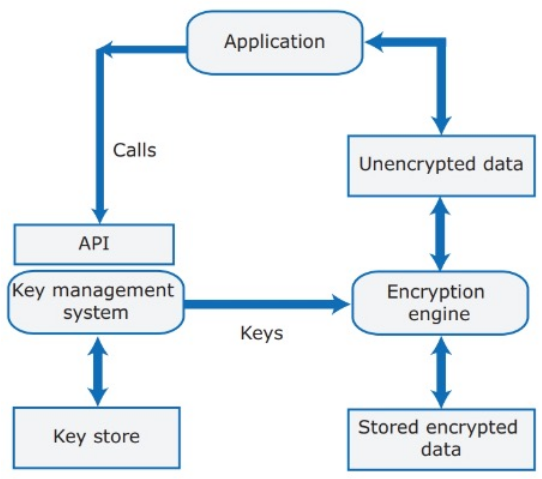
\includegraphics[width=0.70\linewidth,height=0.45\textheight,keepaspectratio]{images/07-sicurezza_fig7-6_kms.png}
\caption{Schema d'uso di un KMS.}
\end{figure}

\section{Privacy}\label{privacy}

\begin{boxdefinition}{Privacy}

La \textbf{privacy} è un concetto sociale che riguarda la raccolta, la
diffusione e l'uso corretto delle informazioni personali possedute da
terzi.

\end{boxdefinition}

\begin{figure}[H]
\centering
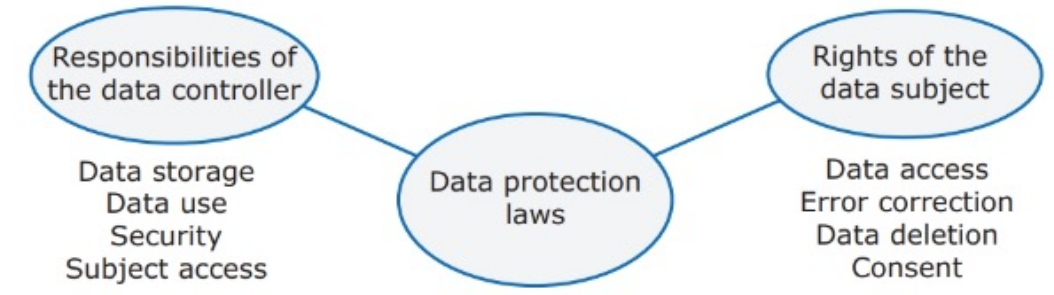
\includegraphics[width=0.90\linewidth,height=0.45\textheight,keepaspectratio]{images/07-sicurezza_fig7-7_leggi-protezione-dati.png}
\caption{Le leggi sulla protezione dei dati.}
\end{figure}

Principi di protezione dei dati (in Europa sono alla base del
\textbf{GDPR}):

\begin{itemize}
\tightlist
\item
  \textbf{Consapevolezza e controllo}: gli utenti devono sapere quali
  dati vengono raccolti mentre usano il prodotto e devono avere il
  controllo sulle informazioni personali raccolte.
\item
  \textbf{Scopo}: bisogna dire agli utenti \textbf{perché} si raccolgono
  i dati, e non usarli per altri scopi.
\item
  \textbf{Consenso}: serve sempre il consenso dell'utente prima di
  comunicare i suoi dati ad altri.
\item
  \textbf{Durata}: non si devono tenere i dati più del necessario. Se un
  utente cancella l'account, vanno cancellati anche i suoi dati
  personali.
\item
  \textbf{Conservazione sicura}: i dati vanno conservati in modo che non
  possano essere alterati o mostrati a persone non autorizzate.
\item
  \textbf{Accesso e correzione}: gli utenti devono poter sapere quali
  dati personali conserviamo e poter correggere eventuali errori.
\item
  \textbf{Luogo}: non si devono conservare i dati in Paesi con leggi
  sulla protezione dei dati più deboli, a meno di un accordo esplicito
  che garantisca regole più forti.
\end{itemize}

Ci sono anche motivi di \textbf{business} per curare la privacy:

\begin{itemize}
\tightlist
\item
  se il sistema non rispetta le leggi sulla protezione dei dati, il
  fornitore rischia cause legali o di non poter vendere il prodotto;
\item
  se il prodotto è venduto ad aziende, i clienti aziendali possono
  pretendere garanzie sulla privacy (per non essere a rischio con i loro
  utenti);
\item
  una fuga o un uso scorretto dei dati dei clienti può danneggiare la
  reputazione del fornitore.
\end{itemize}

Quali dati raccogliere dipende dalle funzionalità del prodotto e dal
modello di business. Altri consigli:

\begin{itemize}
\tightlist
\item
  non raccogliere informazioni personali che non servono;
\item
  definire una \textbf{privacy policy} che dica come vengono raccolte,
  conservate e gestite le informazioni personali e sensibili;
\item
  dire chiaramente se si usano i dati degli utenti per la pubblicità
  mirata o per servizi pagati da altre aziende;
\item
  se il prodotto ha funzioni social con cui gli utenti condividono
  informazioni, assicurarsi che capiscano come controllare cosa
  condividono.
\end{itemize}

\section{Security smell}\label{security-smell}

\subsection{Le sfide della sicurezza nei
microservizi}\label{le-sfide-della-sicurezza-nei-microservizi}

Vediamo le caratteristiche degli attacchi e della sicurezza tipiche dei
microservizi:

\begin{itemize}
\tightlist
\item
  \textbf{Più ampia è la superficie d'attacco, più alto è il rischio}: i
  microservizi si scambiano dati con chiamate remote, quindi ci sono
  potenzialmente moltissimi punti d'ingresso. La sicurezza
  dell'applicazione dipende dall'\textbf{anello più debole}: basta un
  solo punto d'ingresso debole per compromettere tutto.
\item
  \textbf{Controlli di sicurezza distribuiti peggiorano le prestazioni}:
  ogni microservizio deve fare i suoi controlli di sicurezza, magari
  collegandosi a un servizio remoto che rilascia i token. Controlli
  ripetuti e distribuiti rallentano il sistema. Un ripiego è
  \textbf{fidarsi della rete} e saltare i controlli nei singoli
  microservizi, ma la vera soluzione (e la tendenza del settore) è la
  \textbf{rete zero-trust} (non ci si fida di nessuno per default),
  tenendo d'occhio le prestazioni complessive.
\item
  \textbf{Stabilire la fiducia tra microservizi richiede automazione}:
  la comunicazione tra servizi deve avvenire su canali protetti. Se i
  servizi usano certificati, ogni microservizio deve ricevere un
  certificato (e la relativa chiave privata) per autenticarsi con gli
  altri, e chi riceve deve saper validare il certificato di chi chiama.
  Bisogna quindi creare la fiducia tra microservizi, anche revocando e
  rinnovando i certificati. Con centinaia di microservizi serve per
  forza l'\textbf{automazione}.
\item
  \textbf{Tracciare le richieste tra più microservizi è difficile}: i
  \textbf{log} si possono aggregare in metriche che mostrano lo stato
  del sistema (es. media di accessi non validi all'ora) e fanno scattare
  allarmi. Le \textbf{trace} seguono una richiesta da quando entra nel
  sistema a quando esce. A differenza del monolite, una richiesta può
  attraversare molti microservizi, quindi è difficile collegare tra loro
  i pezzi della stessa richiesta.
\item
  \textbf{I container complicano la gestione di credenziali e policy}: i
  container sono server \textbf{immutabili} (ottimo per semplificare il
  deploy e scalare in orizzontale), cioè non cambiano stato dopo
  l'avvio. Ma ogni servizio deve mantenere una lista dinamica di client
  autorizzati e un insieme dinamico di policy di accesso: l'unico modo
  per aggiornarle è tenere le credenziali nel file system del container
  e \textbf{iniettarle all'avvio}.
\item
  \textbf{La distribuzione rende difficile condividere il contesto
  utente}: a una richiesta che si muove nel sistema si vogliono
  associare molte informazioni (es. se è una richiesta premium o no). Il
  problema è far sì che il microservizio che riceve si fidi del contesto
  utente passato da chi chiama (se qualcuno lo manipola, è un attacco).
  Una soluzione diffusa è il \textbf{JSON Web Token (JWT)}, un token di
  sicurezza per condividere il contesto utente tra microservizi.
\item
  \textbf{Le responsabilità di sicurezza sono divise tra team diversi}:
  team indipendenti possono usare tecnologie diverse (buone pratiche di
  sicurezza, strumenti di test di sicurezza statici e dinamici, \ldots).
  Le organizzazioni spesso usano un approccio \textbf{ibrido}: un team
  di sicurezza centrale più esperti di sicurezza dentro i singoli team.
\end{itemize}

\subsection{Smell e refactoring}\label{smell-e-refactoring}

\begin{boxdefinition}{Security smell}

Un \textbf{security smell} è una decisione architetturale di uso comune
che segnala \textbf{possibili violazioni della sicurezza} in
un'applicazione a microservizi.

\end{boxdefinition}

Come per gli architectural smell (vedi
\href{06\%20-\%20Architettura\%20a\%20microservizi}{06 - Architettura a
microservizi}), si vuole capire come rilevarli e risolverli tramite
refactoring, sulla base di una multivocal review. Le proprietà di
sicurezza considerate sono:

\begin{itemize}
\tightlist
\item
  \textbf{Confidenzialità} (\emph{confidentiality}): quanto il sistema
  garantisce che i dati siano accessibili solo a chi è autorizzato.
\item
  \textbf{Integrità} (\emph{integrity}): quanto il sistema impedisce
  modifiche non autorizzate a programmi o dati.
\item
  \textbf{Autenticità} (\emph{authenticity}): quanto si può dimostrare
  che l'identità di un soggetto o di una risorsa è quella dichiarata.
\end{itemize}

Uno smell può violare più proprietà. Ecco gli smell, le proprietà
violate e i refactoring:

\begin{itemize}
\tightlist
\item
  \textbf{Controllo degli accessi insufficiente} (\emph{insufficient
  access control}) --- viola la \textbf{confidenzialità}. Alcuni servizi
  non controllano gli accessi, e questo porta al problema del
  \textbf{confused deputy} (un attaccante ottiene dati a cui non
  dovrebbe accedere, usando un servizio che ha più permessi di lui). I
  permessi del client vanno verificati al momento della richiesta, senza
  aggiungere latenza e colli di bottiglia con chiamate continue a un
  servizio centrale. \textbf{Refactoring}: usare \textbf{OAuth 2.0}, un
  framework basato su token per il controllo degli accessi delegato.
\item
  \textbf{Microservizi accessibili pubblicamente} (\emph{publicly
  accessible microservices}) --- viola la \textbf{confidenzialità}.
  Alcuni microservizi sono raggiungibili direttamente dai client
  esterni: ognuno deve controllare autenticazione e autorizzazione a
  ogni richiesta (più costi di manutenzione) e le credenziali sono più
  esposte. \textbf{Refactoring}: il più citato è un \textbf{API gateway}
  che, da dietro un firewall, gestisce autenticazione, autorizzazione,
  limitazione del traffico e validazione del contenuto dei messaggi.
\item
  \textbf{Privilegi non necessari ai microservizi} (\emph{unnecessary
  privileges}) --- viola \textbf{confidenzialità} e \textbf{integrità}.
  A volte i microservizi hanno livelli di accesso, permessi o
  funzionalità che non servono alle loro funzioni di business, spesso
  perché i programmatori copiano e incollano schemi simili. Più risorse
  esposte senza motivo vuol dire superficie d'attacco più ampia.
  \textbf{Refactoring}: seguire il \textbf{principio del privilegio
  minimo} (\emph{Least Privilege Principle}: il codice deve avere solo i
  permessi necessari per il suo compito, e niente di più).
\item
  \textbf{Crittografia ``fatta in casa''} (\emph{home-made crypto code})
  --- viola \textbf{confidenzialità}, \textbf{integrità} e
  \textbf{autenticità}. Usare codice crittografico scritto da sé può
  essere peggio che non cifrare affatto, per il falso senso di sicurezza
  che dà. \textbf{Refactoring}: usare librerie crittografiche ampiamente
  testate dalla comunità e aggiornate regolarmente (evitando algoritmi
  sperimentali).
\item
  \textbf{Dati esposti non cifrati} (\emph{non-encrypted data exposure})
  --- viola \textbf{confidenzialità}, \textbf{integrità} e
  \textbf{autenticità}. L'applicazione espone per errore dati sensibili
  (es. salvati senza cifratura o con protezioni vulnerabili), e un
  intruso può leggerli o modificarli, credenziali comprese.
  \textbf{Refactoring}: \textbf{cifrare tutti i dati sensibili a
  riposo}; devono restare sempre cifrati ed essere decifrati solo quando
  servono. La maggior parte dei DBMS supporta la cifratura automatica,
  ma si può cifrare anche a livello di applicazione, sistema operativo e
  cache. Attenzione: cifrare consuma risorse, quindi va fatto solo sui
  dati davvero critici.
\item
  \textbf{Segreti scritti nel codice} (\emph{hardcoded secrets}) ---
  viola \textbf{confidenzialità}, \textbf{integrità} e
  \textbf{autenticità}. Segreti come chiavi API, client secret e
  credenziali non vanno mai messi nel codice o nelle variabili
  d'ambiente, perché possono essere esposti per errore (es. un gestore
  di eccezioni che manda informazioni a una piattaforma di logging).
  \textbf{Refactoring}: cifrare i segreti a riposo, non salvare le
  credenziali insieme all'applicazione o nei repository del codice, non
  passare i segreti tramite variabili d'ambiente.
\item
  \textbf{Comunicazione tra servizi non protetta} (\emph{non-secured
  service-to-service communications}) --- viola
  \textbf{confidenzialità}, \textbf{integrità} e \textbf{autenticità}.
  Senza canali sicuri i dati sono esposti ad attacchi
  \textbf{man-in-the-middle}, intercettazione (\emph{eavesdropping}) e
  manomissione (\emph{tampering}). \textbf{Refactoring}: usare il
  \textbf{mutual TLS (mTLS)}, che cifra i dati in transito e ne
  garantisce integrità e riservatezza, e permette a ogni microservizio
  di identificare con certezza l'altro (\textbf{autenticazione
  reciproca}).
\item
  \textbf{Traffico non autenticato} (\emph{unauthenticated traffic}) ---
  viola l'\textbf{autenticità}. I microservizi devono autenticarsi tra
  loro (soprattutto quando si passano il contesto utente). Altrimenti
  sono esposti a manomissione dei dati, denial of service o aumento dei
  privilegi. \textbf{Refactoring}: il \textbf{mutual TLS}, oppure
  \textbf{OpenID Connect}, che usa JWT con le informazioni dell'utente
  autenticato; i microservizi verificano l'identità dell'utente con i
  server di autorizzazione.
\item
  \textbf{Autenticazione multipla} (\emph{multiple user authentication})
  --- viola l'\textbf{autenticità}. È una tentazione far autenticare gli
  utenti da punti diversi, ma ogni punto d'accesso è un possibile varco
  per un intruso. \textbf{Refactoring}: il \textbf{Single Sign-On} (un
  solo punto d'ingresso), che semplifica anche il salvataggio dei log e
  i controlli. Si ottiene con un \textbf{API gateway} e \textbf{OpenID
  Connect} (per condividere il contesto utente).
\item
  \textbf{Autorizzazione centralizzata} (\emph{centralized
  authorization}) --- viola l'\textbf{autenticità}. L'autorizzazione si
  può fare al bordo dell'applicazione (nell'API gateway) e/o in ogni
  microservizio. Se si fa \textbf{solo} al bordo, il punto centrale
  diventa un \textbf{collo di bottiglia}, e c'è il rischio di
  \textbf{confused deputy}: i microservizi si fidano del gateway solo
  perché è il gateway. \textbf{Refactoring}: \textbf{autorizzazione
  decentralizzata}, passando un \textbf{token di accesso} (es. JWT) con
  ogni richiesta a un microservizio e dando accesso solo se il token è
  valido.
\end{itemize}

\subsection{Fare refactoring o no?}\label{fare-refactoring-o-no}

Va deciso \textbf{caso per caso}: risolvere uno smell può peggiorare
altre proprietà! Esempio: passare all'autorizzazione decentralizzata
rispetta i principi di design dichiarati e garantisce le proprietà di
sicurezza, ma quella centralizzata è più facile da mantenere e ha
prestazioni migliori.

Per vedere questi compromessi aiuta modellare le \textbf{interdipendenze
tra obiettivi ``soft''} (\emph{soft goal}) come grafi, che si possono
anche analizzare in modo automatico (Fig. 7.8).

\begin{figure}[H]
\centering
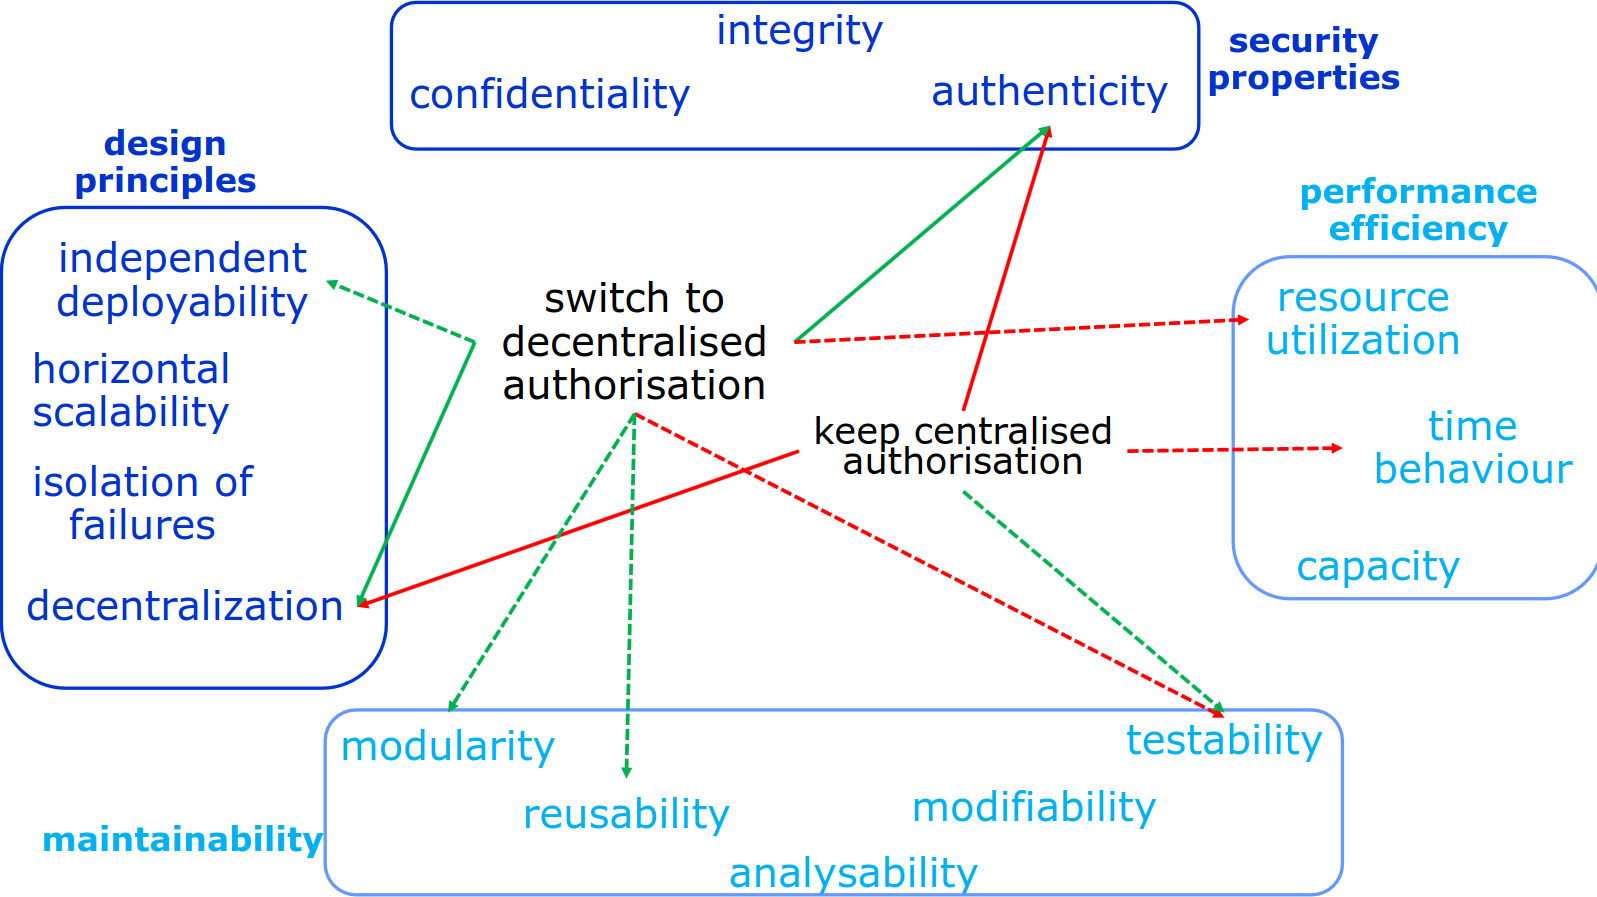
\includegraphics[width=0.79\linewidth,height=0.45\textheight,keepaspectratio]{images/07-sicurezza_fig7-8_autorizzazione-centralizzata.png}
\caption{Confronto tra autorizzazione centralizzata e decentralizzata.}
\end{figure}
